\section{}
The symmetrical frame shown in Fig. \ref{fig:Q5} supports a uniform loading of $p$ per unit length. Assume that each horizontal and vertical
member has the modulus of rigidity $E_1 I_1$ and $E_2 I_2$, respectively. Determine the resultant $R_A$ at the left support, employing
Castigliano's theorem.

\begin{figure}[h]
    \centering
    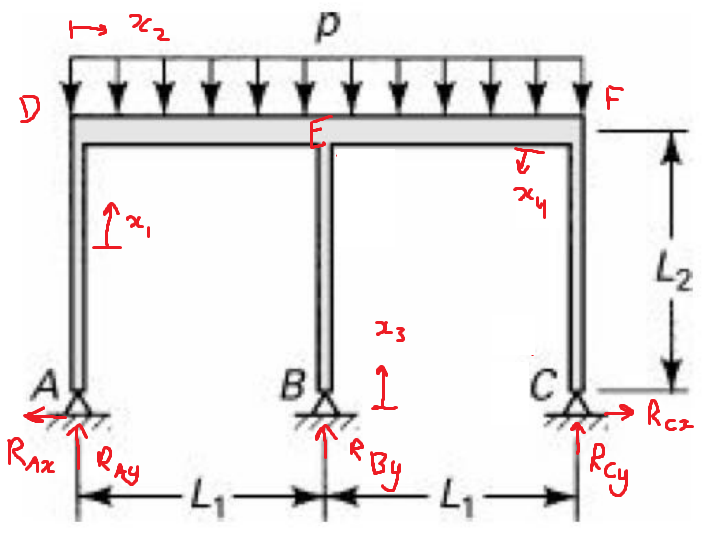
\includegraphics[width=0.5\linewidth]{Questions/Figures/Q5ProblemDiagram.png}
    \caption{Symmetrical frame}
    \label{fig:Q5}
\end{figure}

From A to D, the moment equation is:
\begin{align*}
    M_{AD} &= - R_{Ax} x \\
    \implies \frac{\partial M_{AD}}{\partial R_{Ax}} &= -x
    \implies \frac{\partial M_{AD}}{\partial R_{Ay}} = 0
\end{align*}

From D to F, the moment equation is:
\begin{align*}
    M_{DF} &= M_{AD}|_{x=L_2} + R_{Ay}x - \frac{px^2}{2} \\
    &= -R_{Ax}L_2 + R_{Ay}x - \frac{px^2}{2} \\
    \implies \frac{\partial M_{DF}}{\partial R_{Ax}} &= -L_2 \\
    \implies \frac{\partial M_{DF}}{\partial R_{Ay}} &= x
\end{align*}

From B to E, the moment equation is:
\begin{align*}
    M_{BE} &= 0 \\
    \implies \frac{\partial M_{EB}}{\partial R_{Ax}} &= 0 \\
    \implies \frac{\partial M_{EB}}{\partial R_{Ay}} &= 0
\end{align*}

From C to F, the moment equation is:
\begin{align*}
    M_{CF} &= M_{DF}|_{x=2L_1}  \\ 
    &= -R_{Ax}L_2 + 2R_{Ay}L_1 - 2pL_1^2 \\
    \implies \frac{\partial M_{CF}}{\partial R_{Ax}} &= -L_2 \\
    \implies \frac{\partial M_{CF}}{\partial R_{Ay}} &= 2L_1
\end{align*}

By Castigliano's theorem, the horizontal deflection at A is:
\begin{align*}
    \delta_{A,x} = & \frac{1}{E_1I_1} \left[\int_{0}^{L_2} M_{AD} \left(\frac{\partial M_{AD}}{\partial R_{Ax}}\right) dx
    + \cancel{\int_{0}^{L_2} M_{BE} \left(\frac{\partial M_{BE}}{\partial R_{Ax}}\right) dx}
    + \int_{0}^{L_2} M_{CF} \left(\frac{\partial M_{CF}}{\partial R_{Ax}}\right) dx
    \right] \\
    &+ \frac{1}{E_2I_2} \left[\int_{0}^{2 L_1} M_{DF} \left(\frac{\partial M_{DF}}{\partial R_{Ay}}\right) dx \right] \\
    &= \frac{1}{E_1I_1} \left[\int_{0}^{L_2} R_{Ax} x^2 dx + \int_{0}^{L_2} (-R_{Ax}L_2 + 2R_{Ay}L_1 - 2pL_1^2)(-L_2) dx \right] \\
    &+ \frac{1}{E_2I_2} \left[\int_{0}^{2 L_1} (-R_{Ax}L_2 + R_{Ay}x - \frac{px^2}{2})x dx \right] \\
    &= \frac{1}{E_1I_1} \left[\frac{L_2^3R_{Ax}}{3} + L_2^2(2pL_1^2 - 2R_{Ay}L_1 + L_2R_{Ax}) \right]
    - \frac{1}{E_2I_2} \left[\frac{2pL_1^4}{3} - \frac{2R_{Ay}L_1^3}{3} + \frac{L_2R_{Ax}L_1^2}{2} \right] \\
\end{align*}

Since the pin at A cannot carry deflection, $\delta_{A,x} = 0$. Therefore,
\begin{align*}
    \delta_{A,x} \overset{\text{set}}{=} 0 \\
    \implies R_{Ax} &= -\frac{\frac{L_{2}^2 (2 L_{1}^2 - 2L_1 R_{Ay})}{E_1 I_1} + \frac{\frac{8L_{1}^3 R_{Ay}}{3} - \frac{2L_{1}^4 p}{3}}{E_2 I_2}}
    {\frac{4L_{2}^3}{3 E_1 I_1} - \frac{2L_{1}^2 L_{2}}{E_2 I_2}} 
\end{align*}
By Castigliano's theorem, the vertical deflection at A is:
\begin{align*}
    \delta_{A, y} = &\frac{1}{E_1I_1} \left[\cancel{\int_{0}^{L_2} M_{AD} \left(\frac{\partial M_{AD}}{\partial R_{Ay}}\right) dx}
    + \cancel{\int_{0}^{L_2} M_{BE} \left(\frac{\partial M_{BE}}{\partial R_{Ay}}\right) dx}
    + \int_{0}^{L_2} M_{CF} \left(\frac{\partial M_{CF}}{\partial R_{Ay}}\right) dx
    \right] \\
    &+ \frac{1}{E_2I_2} \left[\int_{0}^{2 L_1} M_{DF} \left(\frac{\partial M_{DF}}{\partial R_{Ay}}\right) dx \right] \\
    &= \frac{1}{E_1I_1} \left[\int_{0}^{L_2} (-R_{Ax}L_2 + 2R_{Ay}L_1 - 2pL_1^2)(2L_1) dx \right]
    + \frac{1}{E_2I_2} \left[\int_{0}^{2 L_1} (-R_{Ax}L_2 + R_{Ay}x - \frac{px^2}{2})(x) dx \right] 
\end{align*}
Too much algebra, by Matlab Symbolic Toolbox:
\begin{verbatim}
ans = 

struct with fields:

Rax: (3*E1*I1*L1^2*p*(2*L1^2 + L2*L1))/(L2*(6*E1*I1*L1^2 + E1*I1*L1*L2 - 3*E2*I2*L2^2))
Ray: (3*L1*p*(3*E1*I1*L1^2 + E1*I1*L1*L2 - E2*I2*L2^2))/...
(6*E1*I1*L1^2 + E1*I1*L1*L2 - 3*E2*I2*L2^2)
\end{verbatim}
The script was used to aid in this solution:
\begin{verbatim}
clc; clear; close all;
syms x L1 L2 p Rax Ray E1 I1 E2 I2
delta_Ax = (1/(E1*I1)) * (int(Rax*x^2, x, 0, L2) + int((-Rax*L2 + 2*Ray*L1 - 2*p*L1^2)*(-L2)...
    , x, 0, L2)) + (1/(E2*I2)) * (int((-Rax*L2 + Ray*x - (p*x^2)/2)*x, x, 0, 2*L1))

delta_Ay = (1/(E1*I1)) * (int((-Rax*L2 + 2*Ray*L1 - 2*p*L1^2)*(2*L1), x, 0, L2)) ...
    + (1/(E2*I2)) * (int((-Rax*L2 + Ray*x - (p*x^2)/2)*(x), x, 0, 2*L1))

eqn1 = delta_Ax == 0;
eqn2 = delta_Ay == 0;
solve(eqn1, Rax)
solve([eqn1, eqn2], [Rax, Ray])
\end{verbatim}